% Copyright 2004 by Till Tantau <tantau@users.sourceforge.net>.
%
% In principle, this file can be redistributed and/or modified under
% the terms of the GNU Public License, version 2.
%
% However, this file is supposed to be a template to be modified
% for your own needs. For this reason, if you use this file as a
% template and not specifically distribute it as part of a another
% package/program, I grant the extra permission to freely copy and
% modify this file as you see fit and even to delete this copyright
% notice. 

\documentclass{beamer}

% There are many different themes available for Beamer. A comprehensive
% list with examples is given here:
% http://deic.uab.es/~iblanes/beamer_gallery/index_by_theme.html
% You can uncomment the themes below if you would like to use a different
% one:
%\usetheme{AnnArbor}
%\usetheme{Antibes}
%\usetheme{Bergen}
%\usetheme{Berkeley}
%\usetheme{Berlin}
%\usetheme{Boadilla}
%\usetheme{boxes}
%\usetheme{CambridgeUS}
%\usetheme{Copenhagen}
%\usetheme{Darmstadt}
%\usetheme{default}
%\usetheme{Frankfurt}
%\usetheme{Goettingen}
%\usetheme{Hannover}
%\usetheme{Ilmenau}
%\usetheme{JuanLesPins}
%\usetheme{Luebeck}
%\usetheme{Madrid}
%\usetheme{Malmoe}
%\usetheme{Marburg}
%\usetheme{Montpellier}
%\usetheme{PaloAlto}
%\usetheme{Pittsburgh}
%\usetheme{Rochester}
%\usetheme{Singapore}
%\usetheme{Szeged}
%\usetheme{Warsaw}
\usetheme{metropolis}

\title{Opening the Black Box of Deep Neural Networks via Information}

% A subtitle is optional and this may be deleted
\subtitle{A paper by Ravid Schwarz-Ziv and Naftali Tishby}

\author{Jani Anttonen}
% - Give the names in the same order as the appear in the paper.
% - Use the \inst{?} command only if the authors have different
%   affiliation.

\institute[] % (optional, but mostly needed)
{
  Department of Future Technologies\\
  University of Turku
}
% - Use the \inst command only if there are several affiliations.
% - Keep it simple, no one is interested in your street address.

\date{17.4.2018}
% - Either use conference name or its abbreviation.
% - Not really informative to the audience, more for people (including
%   yourself) who are reading the slides online

% If you have a file called "university-logo-filename.xxx", where xxx
% is a graphic format that can be processed by latex or pdflatex,
% resp., then you can add a logo as follows:

% \pgfdeclareimage[height=0.5cm]{university-logo}{university-logo-filename}
% \logo{\pgfuseimage{university-logo}}

% Let's get started
\begin{document}

\begin{frame}
  \titlepage
\end{frame}

\begin{frame}{Outline}
  \tableofcontents
  % You might wish to add the option [pausesections]
\end{frame}

% Section and subsections will appear in the presentation overview
% and table of contents.
\section{Background}

\subsection{Motivation for the Paper}

\begin{frame}{Motivation for the Paper}
  \begin{itemize}
  \item {
    There hasn't been a clear reason why deep neural networks \textbf{are generalizing} as well as they do.
  }
  \item {
    \textit{DNNs} don't seem to have an overfitting problem.
  }
  \pause
  \item {
    ...and there's a paper specifying a \textbf{maximal learning bound} named the \textbf{information bottleneck} for neural networks, written by the same \textit{Tishby} as the paper presented here.
  }
  \end{itemize}
\end{frame}

\subsection{Theory}

\begin{frame}{Theory -- Machine Learning}
  \begin{itemize}
  \item {
    The act of distilling the \textbf{essence of information} from data (semi)automatically.
  }
  \pause
  \item {
    In other words, trying to reproduce or \textit{reverse-engineer the function} that would output the same results that exist in the data the algorithm is given.
  }
  \end{itemize}
\end{frame}

\begin{frame}{Theory -- Information Theory}
  \begin{itemize}
  \item {
    Aims to measure how much information can a \textbf{thing} (yes, everything) contain.
  }
  \item {
    Specific implementations include error correction, \alert{compression}, RNGs and cryptoanalysis.
  }
  \end{itemize}
\end{frame}

\begin{frame}{Theory -- Information Theory -- Mutual Information}
  \centering
    \begin{Mutual information is a way to measure how similar two samples of data are.}
        I(x,y) = \sum_{x,y} P(x,y) \ln {{P(x,y)}\over{P(x) P(y)}}
    \end{Mutual information is a way to measure how similar two samples of data are.}
    
  \begin{itemize}
    
    \item {
        \alert{Mutual information} is defined with two entropies, shannon entropy and conditional entropy.
    }
    
    \item {
        It is a very robust \textit{measurement of similarity}.
    }

  \end{itemize}
\end{frame}

\subsection{Looking at Neurons}

\begin{frame}{Looking at Neurons}
  \begin{itemize}
  \item {
    Last layer weights of a network -- Closest representations of the classes
  }
  \item {
    In bigger networks, \alert{weights are somewhat recognizable}. For example, in the case of Google's deep dream, they feed the network back the weights of the last neuron representing a dog, \textit{and get snouts and drooping tongues everywhere}.
  }
  \end{itemize}
\end{frame}

\begin{frame}{Looking at Neurons}
\centering
  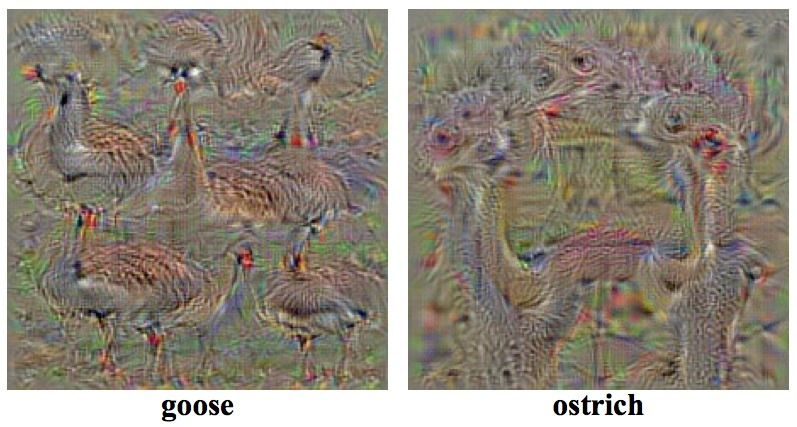
\includegraphics[scale=0.7]{deepvis_goose_ostrich.jpg}
  \cite{DeepVis}
\end{frame}

\begin{frame}{Looking at Neurons}
  \begin{itemize}
  \item {
    By iterating through a number of layers with filters, you \textbf{lose data on every one}.
  }
  \item {
    So what's basically happening is \alert{lossful compression} of the whole input data!
  }
  \end{itemize}
\end{frame}

%% SECOND SECTION %%

\section{Findings}


\subsection{Best-case Scenario}

\begin{frame}{Best-case Scenario}
    \begin{columns}
        \column{0.4\textwidth}
            \begin{enumerate}
                \item {
                    Network copies the training data, gaining information of the data and the labels
                }
                \item {
                    When the gradient gets smaller and smaller it starts to slowly lose information of the original training data, compressing the representation!
                }
            \end{enumerate}
        \column{0.6\textwidth}
            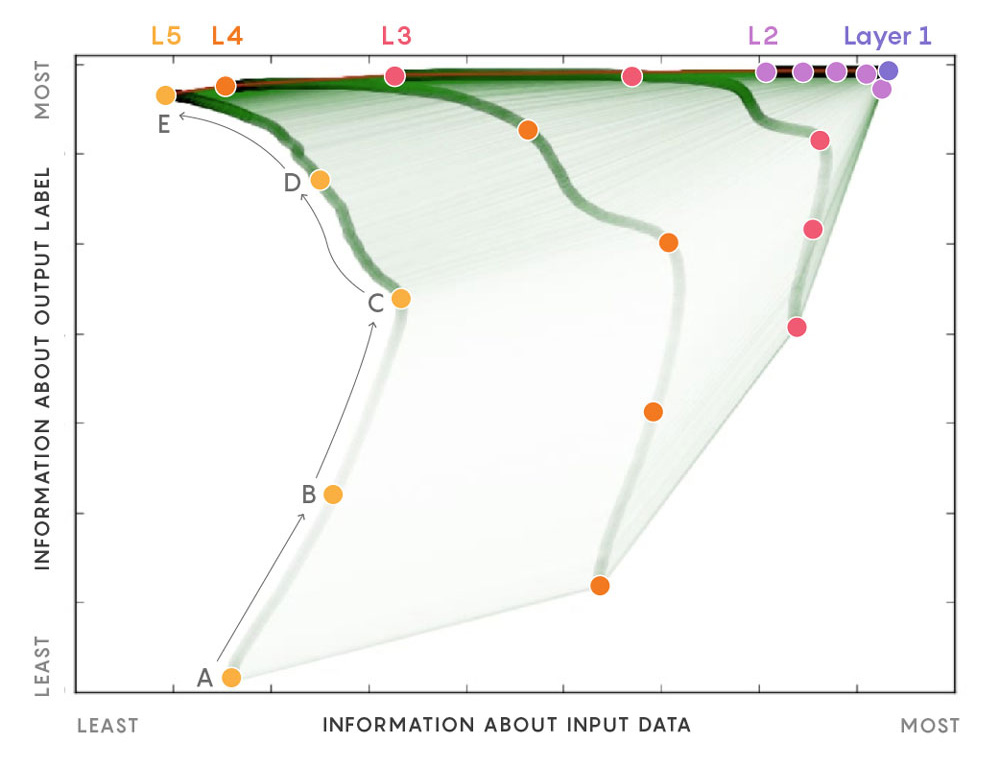
\includegraphics[scale=0.4]{DeepLearning_5001_crop.jpg}
            \cite{Article}
    \end{columns}
\end{frame}

\begin{frame}{Best-case Scenario}
    \centering
        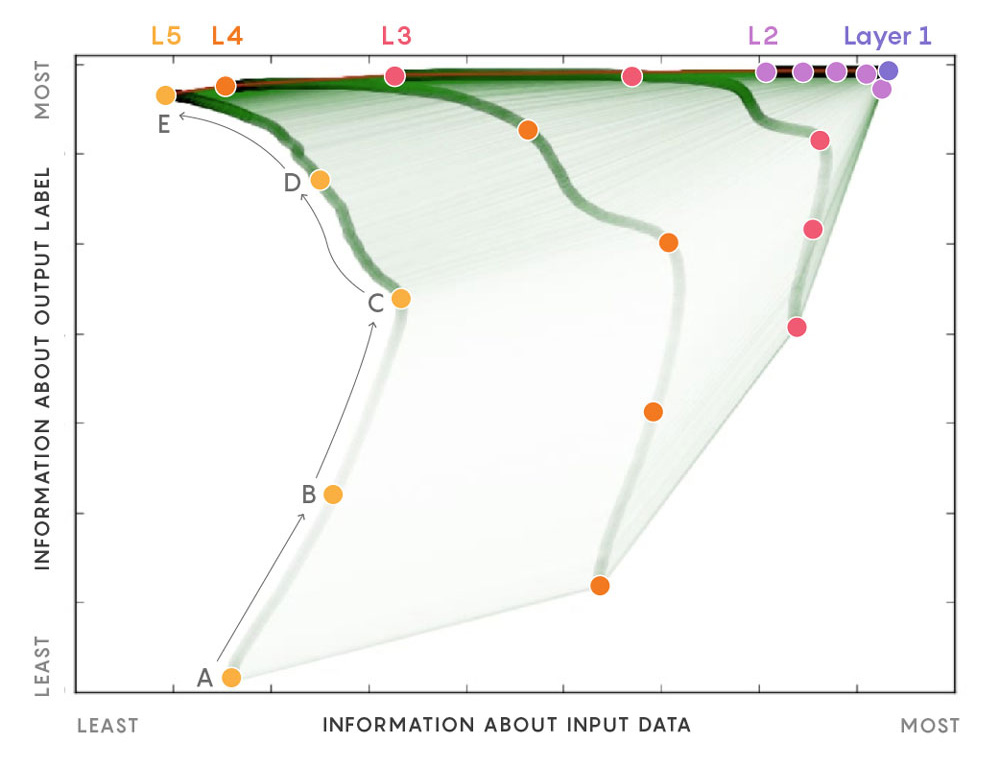
\includegraphics[scale=0.6]{DeepLearning_5001_crop.jpg}
        \cite{Article}
\end{frame}

\begin{frame}{Video Time}
    \centering
        \href{https://www.youtube.com/embed/q45lPv9rev0?enablejsapi=1}{Animation of the training progress in the information plane} \cite{Presentation}
\end{frame}


\subsection{Why Does the Phase Change Happen?}

\begin{frame}{Why Does the Phase Change Happen?}
    \begin{itemize}
        \item \alert{Stochastic gradient descent} adds noise to the signal after a shallow gradient is reached.
        \pause
        \item This noise effectively \textit{wipes out the irrelevant information} of the class, \textbf{compressing} the representation by relaxing the weights.
    \end{itemize}
\end{frame}

\begin{frame}{Why Does the Phase Change Happen?}
    \centering
        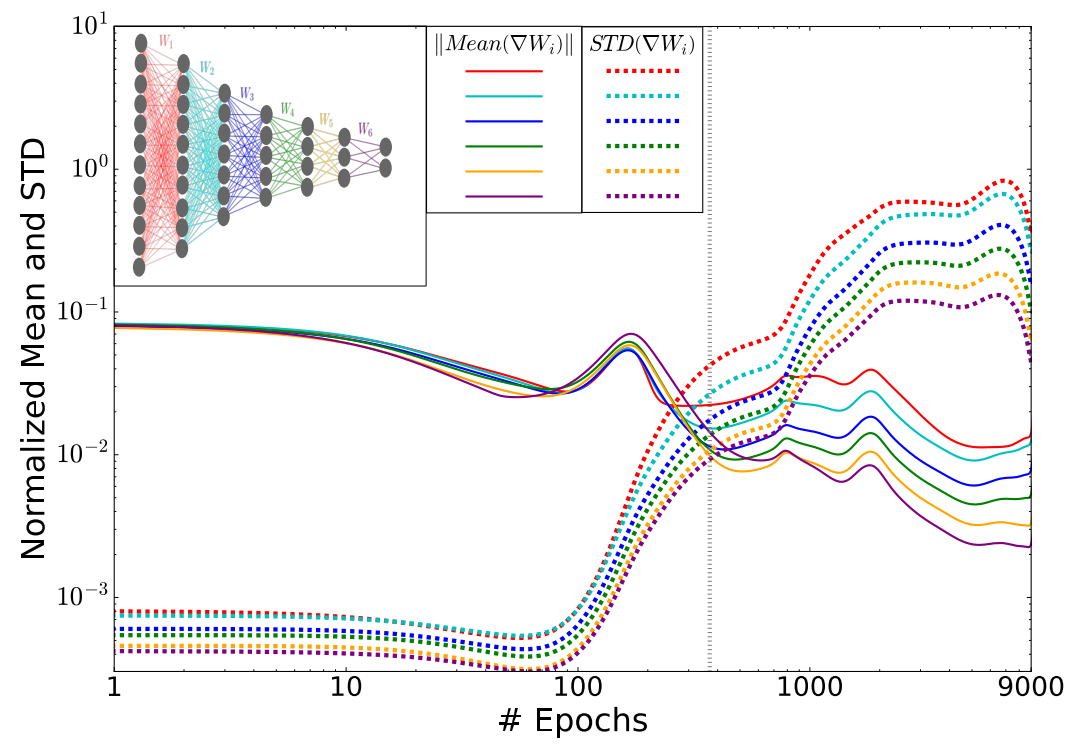
\includegraphics[scale=0.35]{Screenshot_11.png}
        \cite{Paper}
\end{frame}


\subsection{Training Gone Wrong}

\begin{frame}{Training Gone Wrong}
    \begin{columns}
        \column{0.4\textwidth}
            \begin{itemize}
                \item The network \alert{copies} the data well, but fails to generalize because it starts to lose information on the labels when compressing the representation on \textbf{shallow gradients}.
                \item Case: Too little data.
            \end{itemize}
        \column{0.6\textwidth}
            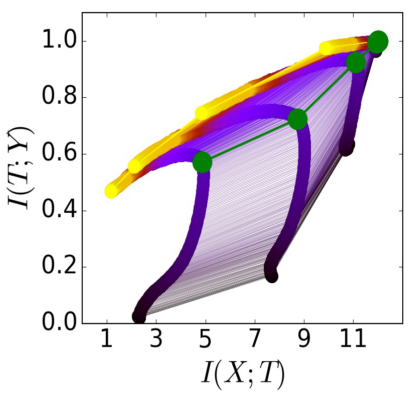
\includegraphics[scale=0.6]{Screenshot_10.png}
            \cite{Paper}
    \end{columns}
\end{frame}


\subsection{More Layers}

\begin{frame}{More Layers = Better Performance AND Speed}
    \centering
        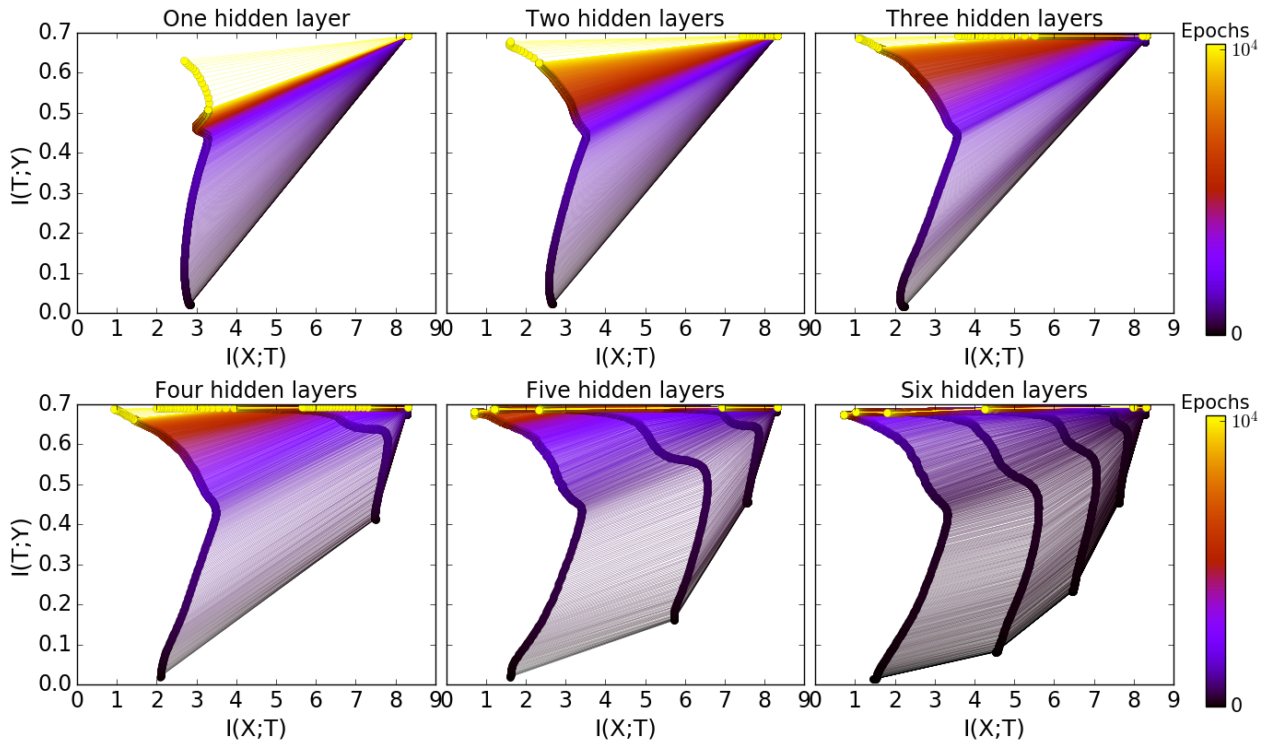
\includegraphics[scale=0.3]{Screenshot_13.png}
        \cite{Paper}
\end{frame}

%% SUMMARY %%

\section{Summary}

\begin{frame}{Summary}
  \begin{itemize}
  \item
    The paper helps us better understand with intuition and theory, what happens during training in modern neural networks.
    \pause
  \item
    This might help us to define better hyperparameters (learning rate and such) for the network beforehand.
    \pause
  \item
    In addition, the information bottleneck bound could be helpful in deciding if you need more data or a better network for a task.
  \end{itemize}
\end{frame}



% All of the following is optional and typically not needed. 
\appendix
\section<presentation>*{\appendixname}
\subsection<presentation>*{Sources}

\begin{frame}[allowframebreaks]
  \frametitle<presentation>{Sources}
    
  \begin{thebibliography}{10}
 
    
  \beamertemplatearticlebibitems
  % Followed by interesting articles. Keep the list short. 

  \bibitem{Paper}
    Schwartz-Ziv, Ravid and Tishby, Naftali
    \newblock Opening the Black Box of Deep Neural Networks via Information
    \newblock {\em arXiv:1703.00810v3},
    2017.
    
  \bibitem{Presentation}
    Tishby, Naftali
    \newblock Presentation: Information Theory of Deep Learning. Naftali Tishby
    \newblock {\em \url{https://www.youtube.com/watch?v=bLqJHjXihK8}},
    2017.
    
  \bibitem{Article}
    Wolchover, Natalie
    \newblock New Theory Cracks Open the Black Box of Deep Learning
    \newblock {\em Quanta Magazine}, Wired to Learn: The Next AI
    2017.
    
  \bibitem{DeepVis}
    Jason Yosinski, Jeff Clune, Anh Nguyen, Thomas Fuchs, Hod Lipson
    \newblock Understanding Neural Networks Through Deep Visualization
    \newblock {\em \url{http://yosinski.com/deepvis}},
    2015.

  \end{thebibliography}
\end{frame}

\end{document}


